\documentclass[10pt, AMS Euler]{article}
\textheight=9.25in \textwidth=7in \topmargin=-.75in
 \oddsidemargin=-0.25in
\evensidemargin=-0.25in
\usepackage{url}  % The bib file uses this
\usepackage{graphicx} %to import pictures
\usepackage{amsmath, amssymb}
\usepackage{theorem, concrete, multicol, color, wasysym}
\usepackage{listings}
\usepackage{float}
\usepackage{color}
\usepackage{bm}

\definecolor{dkgreen}{rgb}{0,0.6,0}
\definecolor{gray}{rgb}{0.5,0.5,0.5}
\definecolor{mauve}{rgb}{0.58,0,0.82}

\lstset{frame=tb,
  language=c++,
  aboveskip=3mm,
  belowskip=3mm,
  showstringspaces=false,
  columns=flexible,
  basicstyle={\small\ttfamily},
  numbers=none,
  numberstyle=\tiny\color{gray},
  keywordstyle=\color{blue},
  commentstyle=\color{dkgreen},
  stringstyle=\color{mauve},
  breaklines=true,
  breakatwhitespace=true,
  tabsize=3
}


\setlength{\intextsep}{5mm} \setlength{\textfloatsep}{5mm}
\setlength{\floatsep}{5mm}


{\theorembodyfont{\rmfamily}
\newtheorem{definition}{Definition}[section]}
{\theorembodyfont{\rmfamily} \newtheorem{example}{Example}[section]}
{\theorembodyfont{\rmfamily} \newtheorem{lemma}{Lemma}[section]}
{\theorembodyfont{\rmfamily} \newtheorem{theorem}{Theorem}[section]}
{\theorembodyfont{\rmfamily} \newenvironment{proof}{\par{\it
Proof:}}{\nopagebreak[4]\rule{2mm}{2mm}}}

%%%%  SHORTCUT COMMANDS  %%%%
\newcommand{\ds}{\displaystyle}
\newcommand{\Z}{\mathbb{Z}}
\newcommand{\arc}{\rightarrow}
\newcommand{\R}{\mathbb{R}}
\newcommand{\N}{\mathbb{N}}
\newcommand{\Q}{\mathbb{Q}}

\newcommand{\stirling}[2]{\genfrac{\{}{\}}{0pt}{}{#1}{#2}}

%%%%  footnote style %%%%

\renewcommand{\thefootnote}{\fnsymbol{footnote}}
\usepackage[utf8]{inputenc}
 
\pagenumbering{roman}

\begin{document}
\noindent{\bf \large ECE 3620 -- Programming Assignment 1}, 10/05/2022, Kade Howes, A02298066\\

\noindent \underline{\hspace{7in}}\\
\section*{1.}
\textit{The program should be written in C or C++. Only libraries from the C/C++ standard libraries
are permitted. No other external libraries should be used – you are writing the entire program from
scratch. You must write all of the code necessary for the processing.}

View AppendixA for C++ code.

\noindent \underline{\hspace{7in}}\\
\section*{2.}
\textit{for the differential equation}
\begin{center}
    \begin{align*}
        (D + 2.5)y_0(t) = 0
    \end{align*}
\end{center}

\textit{with initial condition $y_0(0) = 3$:}

\subsection*{2a}

\textit{Find and plot the analytical (exact) solution to the differential equation for $0 \le t \le 10$.}

From the characteristic equation:
\begin{center}
    \begin{align*}
        \lambda + 2.5 = 0
    \end{align*}
\end{center}

We know $\lambda = -2.5$. So the form for the solution $y_0(t)$ is: 
\begin{center}
    \begin{align*}
        y_0(t) = Ce^{-2.5t}
        \implies C = y_0(0) = 3
        \implies y_0(t) = 3e^{-2.5t}
    \end{align*}
\end{center}

This result in a plot shown below in Figure 2a: 

\begin{figure}[H]
    \centering
    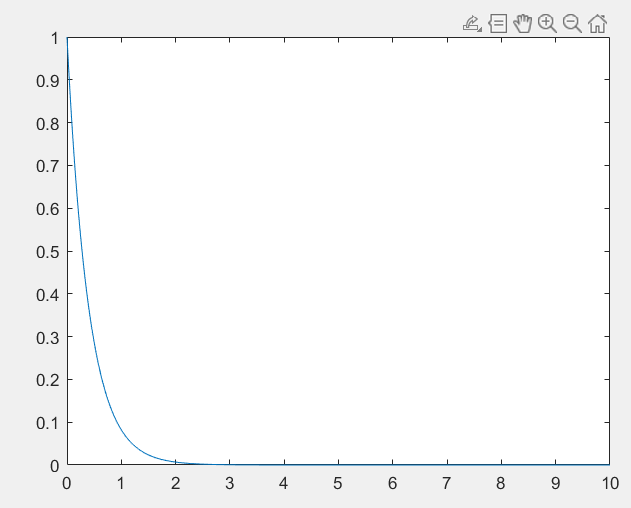
\includegraphics[scale = .5]{analytical2_a.png}\\
    Figure 2a
\end{figure}

\subsection*{2b}
\textit{Write a program in C(++) to plot a numerical solution using (3). You may have to try several
values of $\Delta t$ to get a good enough approximation.}\\

Putting the differential equation and initial condition into my program with a $\Delta t$ of 0.001 results in the plot shown below in Figure 2b:

\begin{figure}[H]
    \centering
    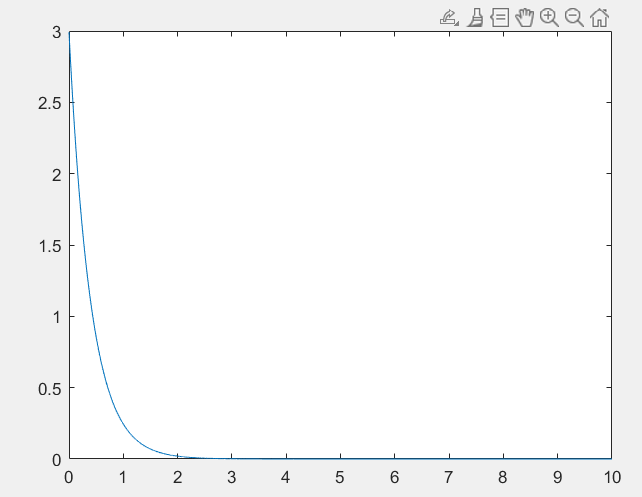
\includegraphics[scale = .5]{programSoln2_a.png}\\
    Figure 2b
\end{figure}

\subsection*{2c}
\textit{Compare the exact solution with the approximate solution.}\\

As seen in the comparison of Figure 2a and Figure 2b, the plot are essentially identical. The approximate solution conformed well to the exact solution.

\noindent \underline{\hspace{7in}}\\
\section*{3.}
\textit{For the third-order differential equation}
\begin{center}
    \begin{align*}
        (D^3 + 0.6D^2 + 25.1125D + 2.5603)y_0(t) = 0
    \end{align*}
\end{center}

\textit{with initial conditions $y_0(0) = 1.5, \dot{y}_0(0) = 2, \ddot{y}_0(0) = -1$:}

\subsection*{3a}

\textit{Find and plot the analytical solution to the differential equation for $0 \le t \le 10$. Identify the roots
of the characteristic equation and plot them in the complex plane}

Using an online cubic root calculator as approved results in the following roots: $\lambda = 0.1, -0.25 \pm 5j$.\\

This results in the form for the solution $y_0(t)$: 
\begin{center}
    \begin{align*}
        y_0(t) = Ce^{-0.1t} + Ae^{-0.25t}\cos{(5t + \theta)}\\
        \implies \dot{y}_0(t) = -0.1Ce^{-0.1t} - 0.25Ae^{-0.25t}\cos{(5t + \theta)} - 5Ae^{-0.25t}\cos{(5t + \theta)}\\
        \implies \ddot{y}_0(t) = 0.01Ce^{-0.1t} + 0.0625Ae^{-0.25t}\cos{(5t + \theta)} + 1.25Ae^{-0.25t}\sin{(5t + \theta)} + \\1.25Ae^{-0.25t}\sin{(5t + \theta)} - 25Ae^{-0.25t}\cos{(5t + \theta)}
    \end{align*}
\end{center}

Which gives us three equations to find the constants $C$, $A$, and $\theta$: 
\begin{center}
    \begin{align*}
        1.5 = C + A\cos{(\theta)}\\
        2 = -0.1C - A\cos{(\theta) - 5A\sin{(\theta)}}\\
        -1 = 0.01C + 0.0625A\cos{(\theta)} + 1.25A\sin{(\theta)} + 1.25A\sin{(\theta)} - 25A\cos{(\theta)}
    \end{align*}
\end{center}

Using a calculator to solve for $C$, $A$, and $\theta$:
\begin{center}
    \begin{align*}
        C = 1.5\\
        A = -0.43\\
        \theta=\frac{\pi}{2}
    \end{align*}
\end{center}

Which holds since $C$ must equal 1.5 and $\theta$ must equal $\frac{\pi}{2}$ by inspection of the numerical plot solution shown later in Figure 3b.

This gives to solution for $y_0(0)$: 

\begin{center}
    \begin{align*}
        y_0(t) = 1.5e^{-0.1t} - 0.43e^{-0.25t}\cos{(5t + \frac{\pi}{2})}
    \end{align*}
\end{center}

Plotting this function results in the plot shown below in Figure 3a.
\begin{figure}[H]
    \centering
    \includegraphics[scale = .6]{analytical3_a.png}\\
    Figure 3a
\end{figure}

Here is the plot of the roots of the characteristic equation on the complex plane:

\begin{figure}[H]
    \centering
    \includegraphics[scale = .5]{complexPlane2.png}
\end{figure}

\subsection*{3b}
\textit{Put the third-order differential equation into state-space form.
}\\

let $x_1(t) = y_0(t)$, $x_2(t) = \dot{y}_0(t)$, and $x_3(t) = \ddot{y}_0(t)$.\\

State-space form should be $\dot{\boldsymbol{x}}(t) = A\boldsymbol{x}(t)$.

\begin{center}
    \begin{align*}
        A = \begin{bmatrix}
        0 & 1 & 0\\
        0 & 0 & 1\\
        -2.5063 & -25.1125 & -0.6
        \end{bmatrix}\\
        \dot{\boldsymbol{x}}(t) = 
        \begin{bmatrix}
        0 & 1 & 0\\
        0 & 0 & 1\\
        -2.5063 & -25.1125 & -0.6
        \end{bmatrix}
        \boldsymbol{x}(t)
    \end{align*}
\end{center}

\subsection*{3c}
\textit{Write a program in C(++) to plot an approximate solution using (8). You may have to try several
values of $\Delta t$ to get a reasonable approximation.}\\

Putting the differential equation and initial conditions into my program with a $\Delta t$ of 0.001 results in the plot shown below in Figure 3b:

\begin{figure}[H]
    \centering
    \includegraphics[scale = .6]{programSoln3_a.png}\\
    Figure 3b
\end{figure}

\subsection*{3d}
\textit{Compare the exact solution with the approximate solution.}\\

As can be seen in the comparison of the plots shown in Figure 3a and Figure 3b, the exact solution and approximate solution are very close. The approximate solution produced by the program was accurate.


\noindent \underline{\hspace{7in}}\\
\section*{4.}
\textit{For the circuit shown here:}
\begin{figure}[H]
    \centering
    \includegraphics[scale = .6]{circuit.png}
\end{figure}

\textit{where $R_1 = 1$ kΩ, $R_2 = 22$ kΩ, $C = 10$ µF, and $L = 5$ H.}






\noindent \underline{\hspace{7in}}\\

\section*{AppendixA}
\b Here is my C++ code to dynamically approximate the solution to any order differential equation (odeSolve.cpp):
\begin{lstlisting}
 #include <iostream>
#include <fstream>

using namespace std;
void getCoefficients(int order, double *coefficients);
void getInitials(int order, double *initials);
float getDeltaT();
float getStartTime();
float getEndTime();
void initializeX(int order, double *x, double *initials);
void initializeA(int order, double dt, double **A, double *coeffiecients);
void matrixVecMult(int order, double **A, double *x, double *newx);

int main() {
    // open file to write output to
    ofstream outfile("output.txt");
    // ask user for the order of differential equation and store in order
    int order = 1;
    cout << "Enter the order of the differential equation: ";
    cin >> order;
    
    // get user input (coefficients, intials, delta t, start time, and end time)
    double coefficients[order];
    getCoefficients(order, coefficients);
    double initials[order];
    getInitials(order, initials);
    float dt = getDeltaT();
    float startTime = getStartTime();
    float endTime = getEndTime();

    // create x vector (start with intial conditions)
    double x[order];
    initializeX(order, x, initials);
    // create matrix I + A(dt)
    double **A;
    A = new double* [order];
    for (int i = 0; i < order; i++) {
        A[i] = new double[order];
    }
    initializeA(order, dt, A, coefficients);

    // set up time and counting variables
    float runTime = startTime - endTime;
    float numPoints = runTime / dt;
    double newx[order];
    for (float t = startTime; t <= endTime; t += dt) {
        matrixVecMult(order, A, x, newx);
        // write newx's x1 to file with time t
        outfile << t << " " << newx[0] << endl;
        // change x = newx for next iteration
        for (int i = 0; i < order; i++) {
            x[i] = newx[i];
        }
    }  

    // close output file 
    outfile.close();
}

void matrixVecMult(int order, double **A, double *x, double *newx) {
    double sum;
    for (int i = 0; i < order; i++) {
        sum = 0;
        for (int j = 0; j < order; j++) {
            sum += A[i][j] * x[j];
        }
        newx[i] = sum;
    }
}

void initializeX(int order, double *x, double *initials) {
    cout << "x vector: \n";
    for (int i = 0; i < order; i++) {
        x[i] = initials[i];
        cout << x[i] << "\n";
    }

}

void initializeA(int order, double dt, double **A, double *coeffiecients) {
    for (int i = 0; i < order; i++) {
        for (int j = 0; j < order; j++) {
            if (j == (i + 1)) {
                A[i][j] = 1;
            }
            // last row
            if (i == (order - 1)) {
                A[i][j] = -1 * coeffiecients[j];
            }
            // multiply by dt
            A[i][j] = A[i][j] * dt;
            // add identity matrix now
            if (i == j) {
                A[i][j] = A[i][j] + 1;
            }
        }
    }

    // print A matrix
    cout << "Matrix I + A(dt):\n";
    for (int i = 0; i < order; i++) {
        for (int j = 0; j < order; j++) {
            cout << A[i][j] << " ";
        }
        cout << "\n";
    }
}


void getCoefficients(int order, double *coefficients) {
    // ask user for constant coeffiecients
    cout << "Enter coefficients from a_" << order-1 << " down to a_0:\n";
    int index = 0;
    for (int i = order-1; i >= 0; i--, index++) {
        cout << "coefficient a_" << i << ": ";
        cin >> coefficients[i];
    }
    // print out coeffients
    cout << "coefficients array: ";
    for (int i = 0; i < order; i++) {
        cout << coefficients[i] << " ";
    }
}

void getInitials(int order, double *initials) {
    cout << "\n\nEnter initial conditions:\n";
    for (int i = 0; i < order; i++) {
        // ask for specific y'(t) inital condition
        cout << "Intial condition for y";
        for (int j = 0; j < i; j++) {
            cout << "'";
        }
        cout << "(t): ";
        cin >> initials[i];
    }

    // print out initial conditions
    cout << "initials array: ";
    for (int i = 0; i < order; i++) {
        cout << initials[i] << " ";
    }
}

float getDeltaT() {
    cout << "\n\nEnter delta t (dt): ";
    float t;
    cin >> t;
    return t;
}

float getStartTime() {
    cout << "\n\nEnter start time: ";
    float t;
    cin >> t;
    return t;
}

float getEndTime() {
    cout << "\n\nEnter end time: ";
    float t;
    cin >> t;
    return t;
}
\end{lstlisting}

\textbf{Important notes}: Make notes like this
\begin{lstlisting}
    Here I put some text files
\end{lstlisting}

\newpage
\noindent \underline{\hspace{7in}}\\

\noindent \underline{\hspace{7in}}\\
\begin{center}
    \begin{align*}
        y_0(t) &= c_1e^{-0.1 t} + c_2e^{-0.25 t}[A \cos{5t} + B \sin{5t}]\\
        \dot{y}_0(t) &= -0.1c_1e^{-0.1 t} \\
        \textit{Here's how you put math into the code.}
    \end{align*}
\end{center}
\textit{Here is how you add a photo.}
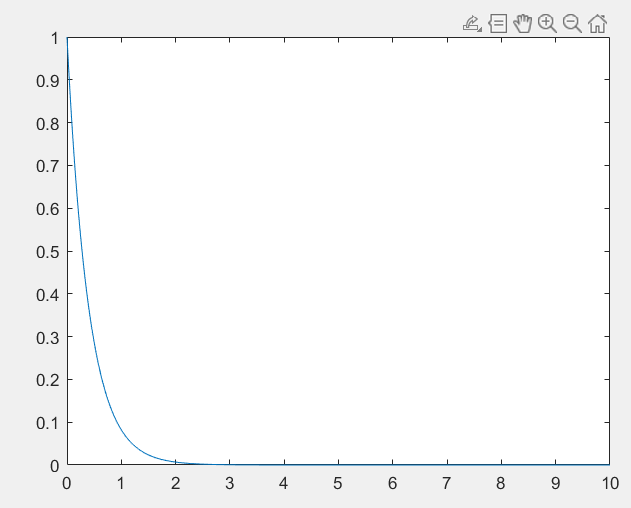
\includegraphics[scale = 1]{analytical2_a.png}
\end{document}